\section{Partitioning}
\subsection{Models for System Synthesis}
\begin{itemize}
	\item Allocation + Binding = Partitioning
	\item Problem graph
\begin{itemize}
	\item Nodes: functional and communication task
	\item Edges: dependencies
\end{itemize}
	\item Architecture graph
\begin{itemize}
	\item Nodes: functional and communication resources
	\item Edges: directed communication resources 
\end{itemize}
	\item Specification graph
\begin{itemize}
	\item Problem graph + Architecture graph + Mapping edges
\end{itemize}
\end{itemize}

\begin{figure}
	\begin{center}
		\begin{subfigure}[b]{0.45\textwidth}
			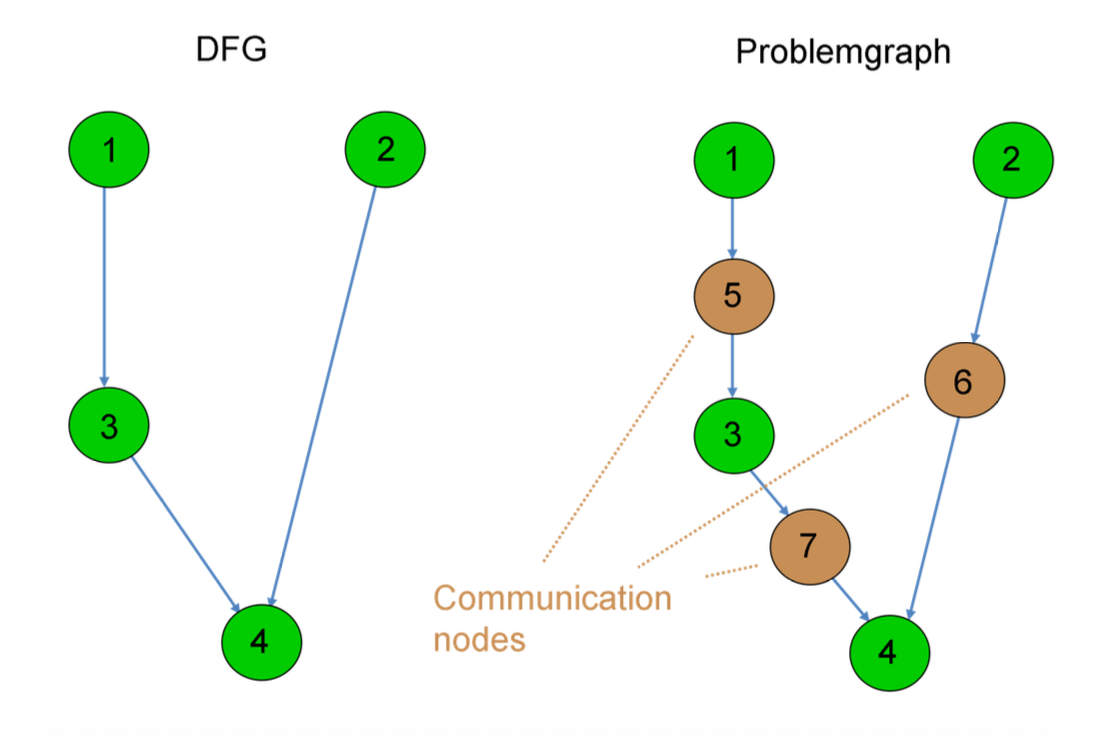
\includegraphics[width=\textwidth]{images/Problem_graph.png}
			\caption{Problem graph}
		\end{subfigure}
		\hfill
		\begin{subfigure}[b]{0.45\textwidth}
			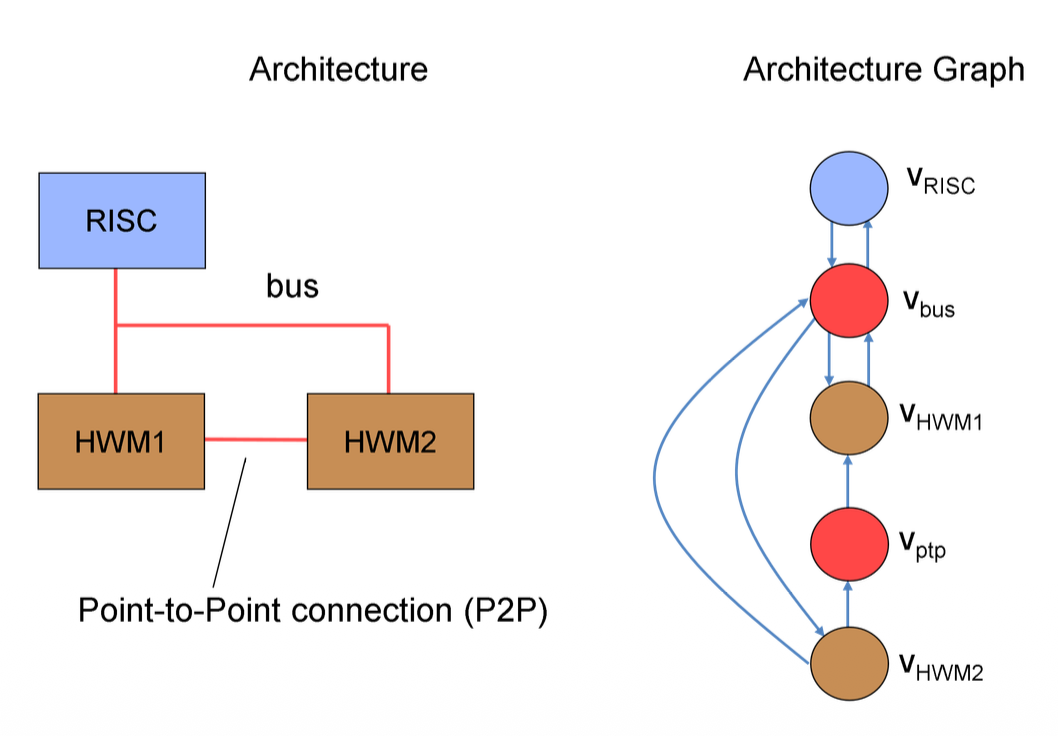
\includegraphics[width=\textwidth]{images/Architecture_graph.png}
			\caption{Architecture graph}
		\end{subfigure}
		\begin{subfigure}[b]{0.45\textwidth}
			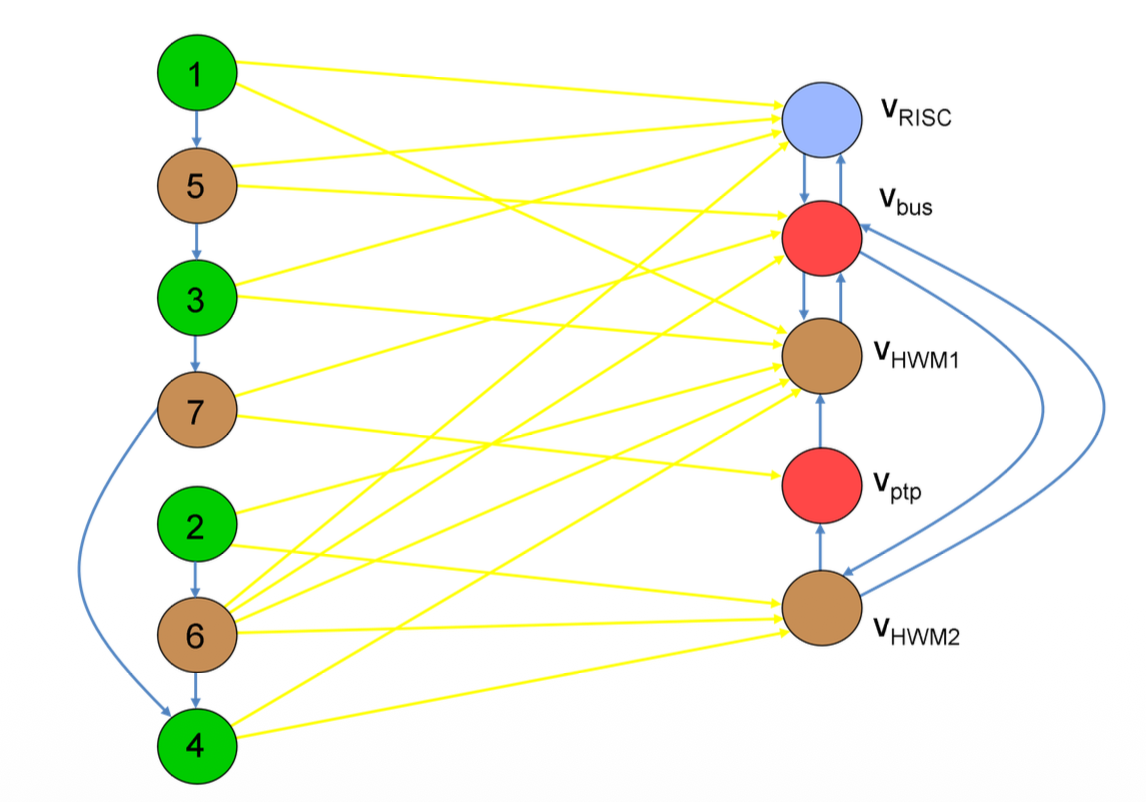
\includegraphics[width=\textwidth]{images/Specification_graph.png}
			\caption{Specification graph}
		\end{subfigure}
		\hfill
		\begin{subfigure}[b]{0.45\textwidth}
			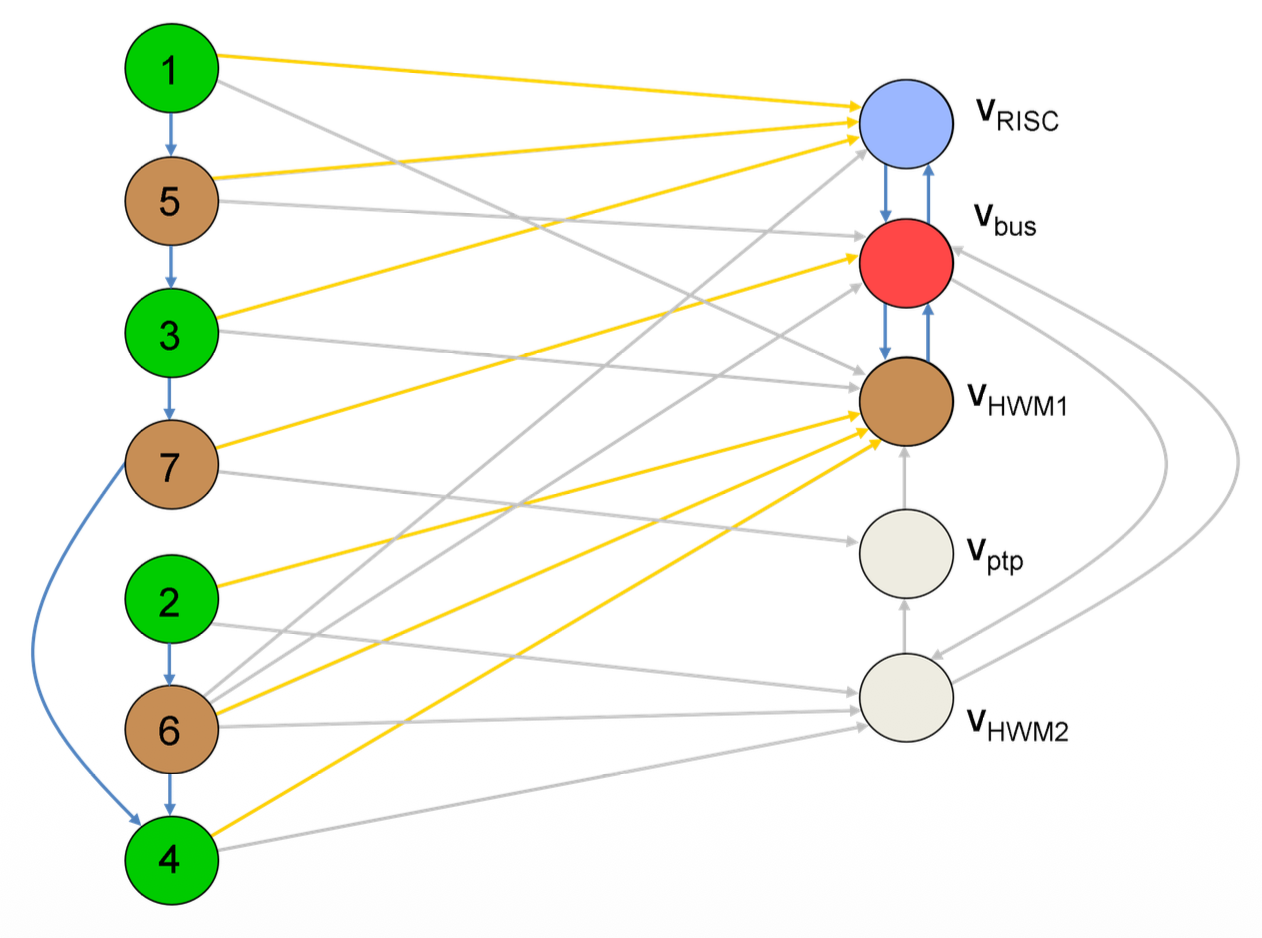
\includegraphics[width=\textwidth]{images/Allocation_binding.png}
			\caption{Allocation and binding}
		\end{subfigure}
		\caption{Models for System Synthesis}
		\label{fig:system_synthesis}
	\end{center}
\end{figure}

\subsection{Partitioning}
\begin{itemize}
	\item Abstraction level
\begin{itemize}
	\item Structural partitioning: RTL, netlists
\begin{itemize}
	\item System relatively well known
	\item No more comparison of design alternatives possible 
\end{itemize}
	\item Functional partitioning: system level
\begin{itemize}
	\item Comparison of design alternatives possible
	\item Quality of designs still not accurate
	$\rightarrow$ Estimation, Rapid Prototyping
\end{itemize}
\end{itemize}
	\item Cost( objective) function - Example:
\begin{itemize}
	\item $f(C, L, P) = k_1 \cdot h_c(C, \overline C) + k_2 \cdot h_L (L, \overline L) + k_3 \cdot h_p(P, \overline P)$
	\item System cost $C$, Latency $L$ and Power consumption $P$ 
\end{itemize}
	\item Problem definition: Group $n$ objects $O = \{o_1, \dots, o_n\}$ into $m$ blocks $P = \{p_1, \dots, p_m\}$ such that
\begin{itemize}
	\item $p_1 \cup \dots \cup p_m = O$
	\item $p_i \cap p_j = \emptyset \quad \forall i, j:i\not = j$
	\item while minimizing the cost $c(P)$
	\item The general partitioning problem is NP-complete
\end{itemize}
\end{itemize}

\subsubsection{General partitioning methods}
\begin{itemize}
	\item Heuristics
\begin{itemize}
	\item Constructive methods
\begin{itemize}
	\item Random mapping
	\item Hierarchical clustering (!!! Bullshit !!!)
\end{itemize}
	\item Iterative improvement methods
\begin{itemize}
	\item Kernighan-Lin algorithm
	\item Simulated Annealing
\end{itemize}
	\item Evolutionary algorithms
\end{itemize}
	\item Exact techniques
\begin{itemize}
	\item Enumeration of solution space
	\item Integer Linear Program (ILP)
\end{itemize}
\end{itemize}

\subsubsection{Constructive Methods}
\begin{itemize}
	\item Random Mapping
\begin{itemize}
	\item Each object is mapped randomly to a block
\end{itemize}
	\item Hierarchical clustering
\begin{itemize}
	\item Stepwise grouping of objects using a closeness function that indicates how beneficial it is to group two objects together
\end{itemize}
	\item Constructive methods
\begin{itemize}
	\item Are often used to fina an initial partition for methods of iterative improvement
	\item Have a problem in defining suitable closeness functions
\end{itemize}
\end{itemize}

\begin{figure}[h]
	\begin{center}
		\begin{subfigure}[b]{0.45\textwidth}
			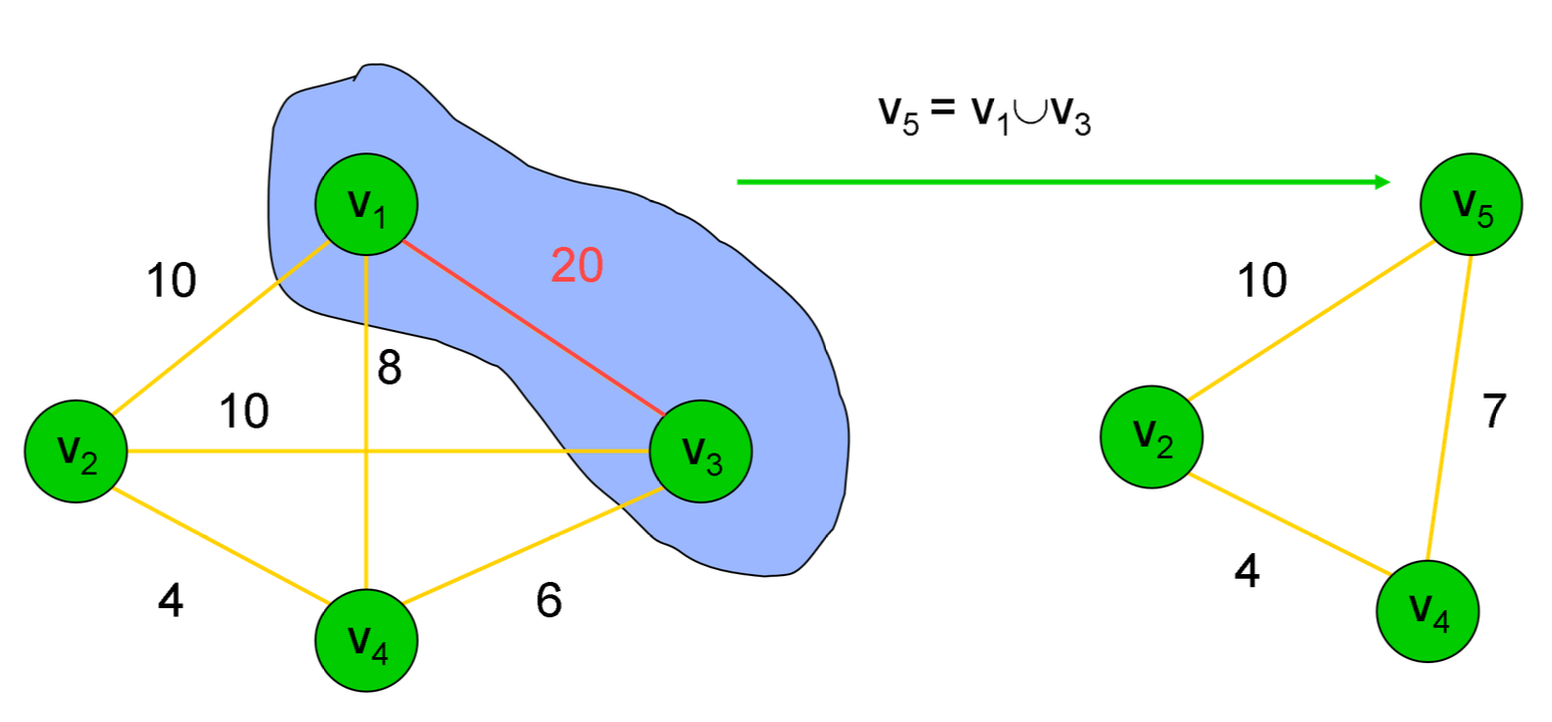
\includegraphics[width=\textwidth]{images/Hierarchical_clustering_1.png}	
		\end{subfigure}
		\hfill
		\begin{subfigure}[b]{0.45\textwidth}
			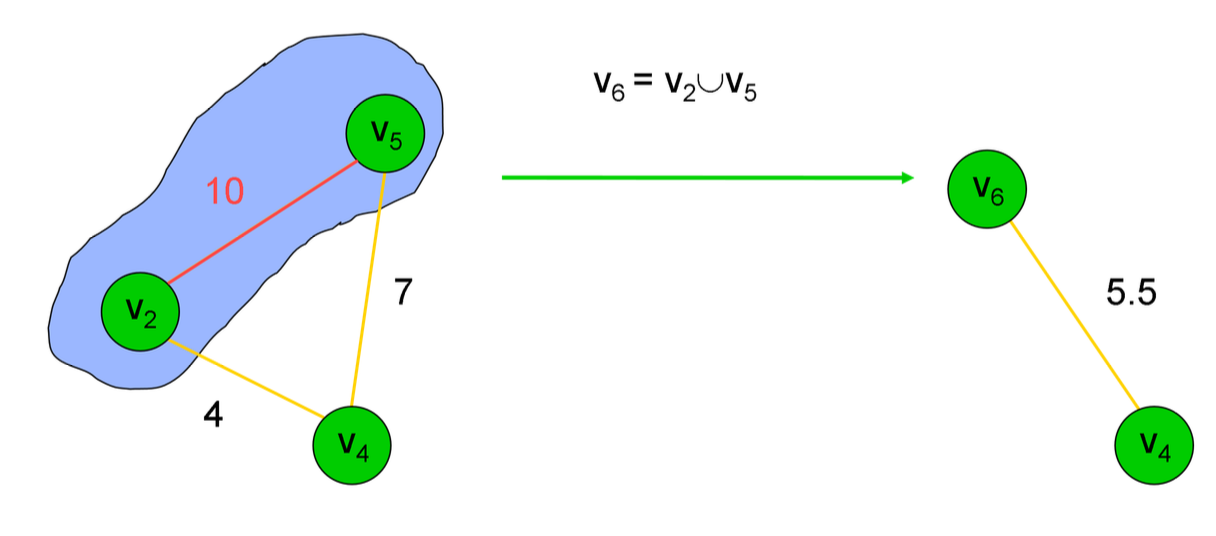
\includegraphics[width=\textwidth]{images/Hierarchical_clustering_2.png}	
		\end{subfigure}
		\begin{subfigure}[b]{0.45\textwidth}
			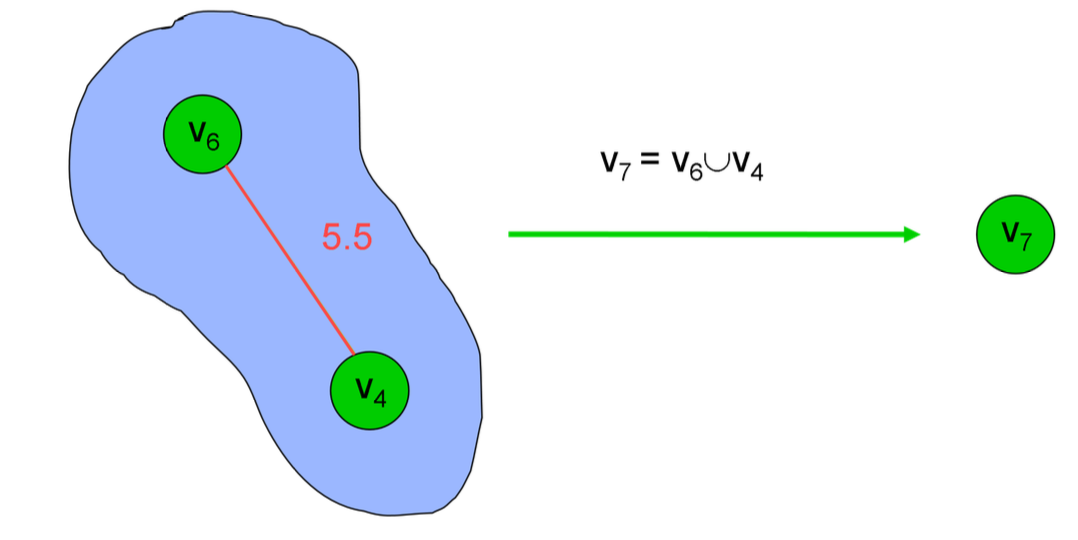
\includegraphics[width=\textwidth]{images/Hierarchical_clustering_3.png}	
		\end{subfigure}
		\hfill
		\begin{subfigure}[b]{0.45\textwidth}
			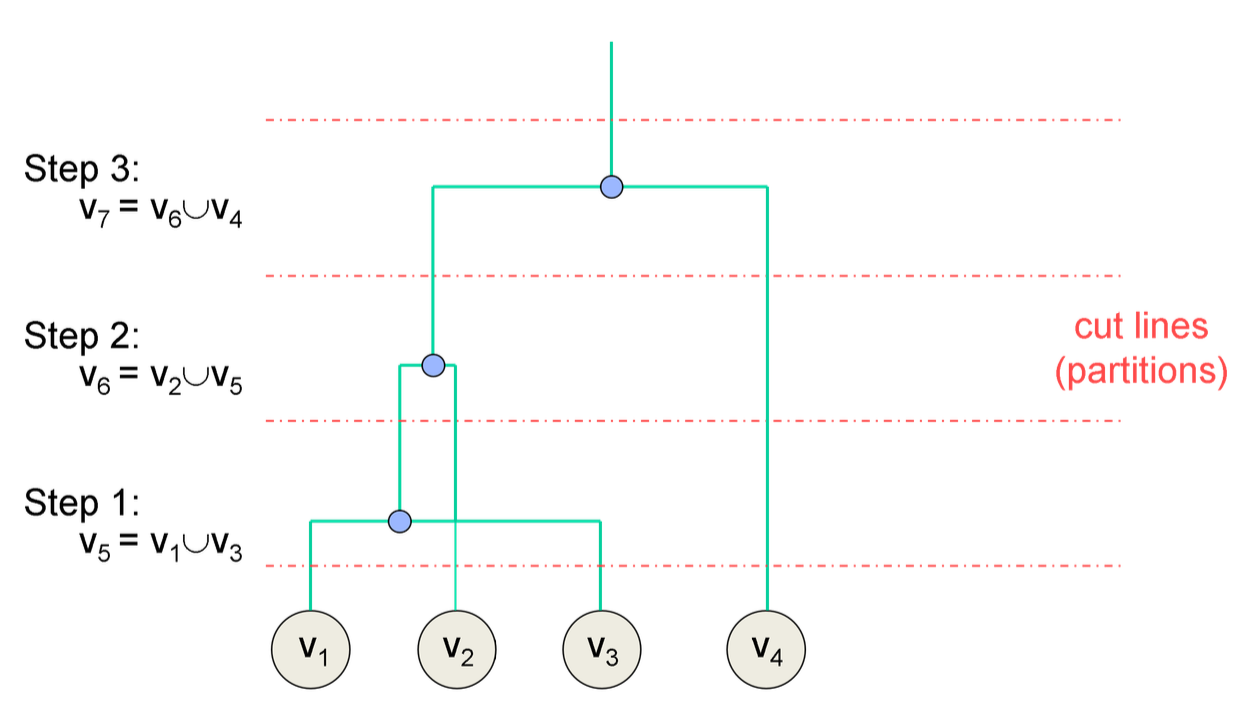
\includegraphics[width=\textwidth]{images/Hierarchical_clustering_4.png}	
		\end{subfigure}
	\end{center}
	\caption{Hierarchical Clustering - Example}
	\label{fig:hierarchical_clustering}
\end{figure}

\subsubsection{Kernighan-Lin Algorithm}
\begin{itemize}
	\item Creation of bi-partitions 
\begin{itemize}
	\item Group the object into the other group that causes the greatest decrease in cost
	\item May escape local minima
	\item As long as abetter partition is found
\begin{itemize}
	\item Tentatively group of the $n$ objects the "best", then from the $n-1$ remaining again, until each object has been re-grouped at least once
	\item From these $n$ partitions, take the one with the minimal cost and perform the respective re-grouping
	\item robust method, in $\BigO(n^2)$
\end{itemize}
	\item Partitioning into $m$ blocks: $\BigO(mn^2)$
\end{itemize}
\end{itemize}

\begin{figure}[h]
	\begin{center}
		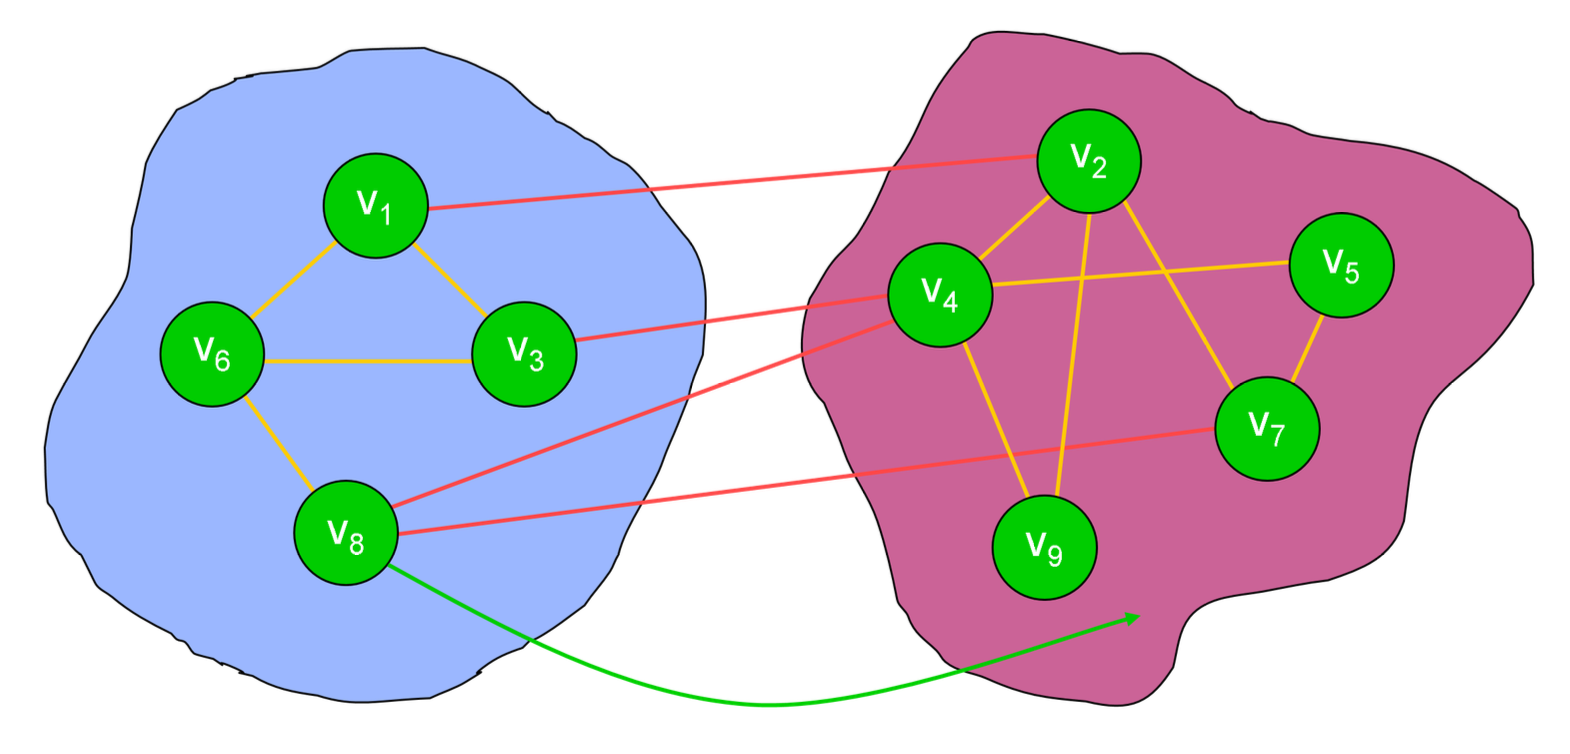
\includegraphics[width=0.5\textwidth]{images/Kernighan-Lin.png}
		\caption{Kernighan-Lin Algorithm}
		\label{fig:Kernighan-Lin}
	\end{center}
\end{figure}

\subsubsection{Simulated Annealing}
\begin{itemize}
	\item Time complexity:
\begin{itemize}
	\item From exponential to constant, depending on the implementation of the functions \textbf{Equilibrium}, \textbf{DecreseTemp} and \textbf{Frozen}
	\item The longer the executions times, the better the results
	\item Goal: polynomial execution time
\end{itemize}
\begin{verbatim}
	 (1)	temp <- temp_start
	 (2) cost <- c(P)
	 (3) while Frozen = false do
	 (4)     while Equilibrium = false do
	 (5)         P' <- RandomMove(P)
	 (6)         cost' <- c(P')
	 (7)         deltacost <- cost' - cost
	 (8)         if Accept(deltacost, temp) > Random(0, 1) then
	 (9)             P <- P'
	(10)             cost <- cost'
	(11)         end if
	(12)     end while
	(13)     temp <- DecreaseTemp(temp)
	(14) end while
\end{verbatim}
\end{itemize}

\subsubsection{Integer Linear Programs}
\begin{itemize}
	\item Conditions are modeled as constraints of the ILP \\
			Example: maximum number $h_k$ of objects in block $p_k$
			$$
				\sum_{i=1}^nx_i,k\leq h_k\quad1\leq k\leq m
			$$ 
	\item ILP is an exact method, NP-complete
	\item may be applied successfully for problems
\begin{itemize}
	\item Of small size
	\item If objective function and constrains are linear
\end{itemize}
\end{itemize}

\subsection{Algorithms for HW/SW-Partitioning}
\begin{itemize}
	\item The easiest problem instance is a bi-partitioning problem $P=\{p_{SW}, p_{HW}\}$
	\item Software-oriented approach: $P=\{O, \emptyset\}$
\begin{itemize}
	\item Easy, as when starting with SW specification, all functions are implementable
	\item Performance constrains may not be satisfied $\rightarrow$ Migration of objects to HW 
\end{itemize}
	\item Hardware-oriented approach: $P=\{\emptyset, O\}$
\begin{itemize}
	\item Performance certainly satisfied if all objects are initially implemented in HW
	\item Cost constrains may not be satisfied $\rightarrow$ Migration of objects to SW
\end{itemize}
\end{itemize}

\subsubsection{Greedy Algorithms}
\begin{itemize}
	\item Migration of objects into the other block until no further improvements observable
\begin{verbatim}
	(1) repeat
	(2)     P_old <- P
	(3)     for i <- 1 to n do
	(4)         if f(MOVE(P, o_i)) < f(P) then
	(5)             P < MOVE(P, o_j)
	(6)         end if
	(7)     end for
	(8) until P = P_old
\end{verbatim}
	\item \verb|f(x)| is cost function
\end{itemize}

\subsection{Basic of Evolutionary Algorithms}
\begin{itemize}
	\item Algorithms that are based on the optimization of evolution
	\item \glqq{}Individual\grqq{} $\rightarrow$ Structure (solution)
	\item \glqq{}Genotype\grqq{} $\rightarrow$ Coded solution (only GAs)
\begin{itemize}
	\item Bit string (search space of size $2^n$)
	\item Integer genotype (search space of size $m^n \quad, m\in\N$)
	\item Double genotype (search space of size $m^n \quad, m\in\R$)
	\item Permutation genotype (search space in list of $n$ objects in search space $n!$) 
\end{itemize}

	\item \glqq{}Phenotype\grqq{} $\rightarrow$ Decoded solution (only GAs)
	\item \glqq{}Population\grqq{} $\rightarrow$ Set of individuals
	\item \glqq{}Fitness\grqq{} $\rightarrow$ Quality of an individual
	\item Evolutionary operators
\begin{itemize}
	\item Selection
	\item Recombination
	\item Mutation
\end{itemize}
\end{itemize}

\subsection{Design space exploration}
\begin{itemize}
	\item Design space $\rightarrow$ Different implementations of a specification
	\item Design point $\rightarrow$ One Implementation
	\item Optimization $\rightarrow$ Determination of the \glqq{}best\grqq{} implementation
	\item Pareto-point $\rightarrow$ Non-dominant design point 
\end{itemize}

\begin{figure}[h]
	\begin{center}
		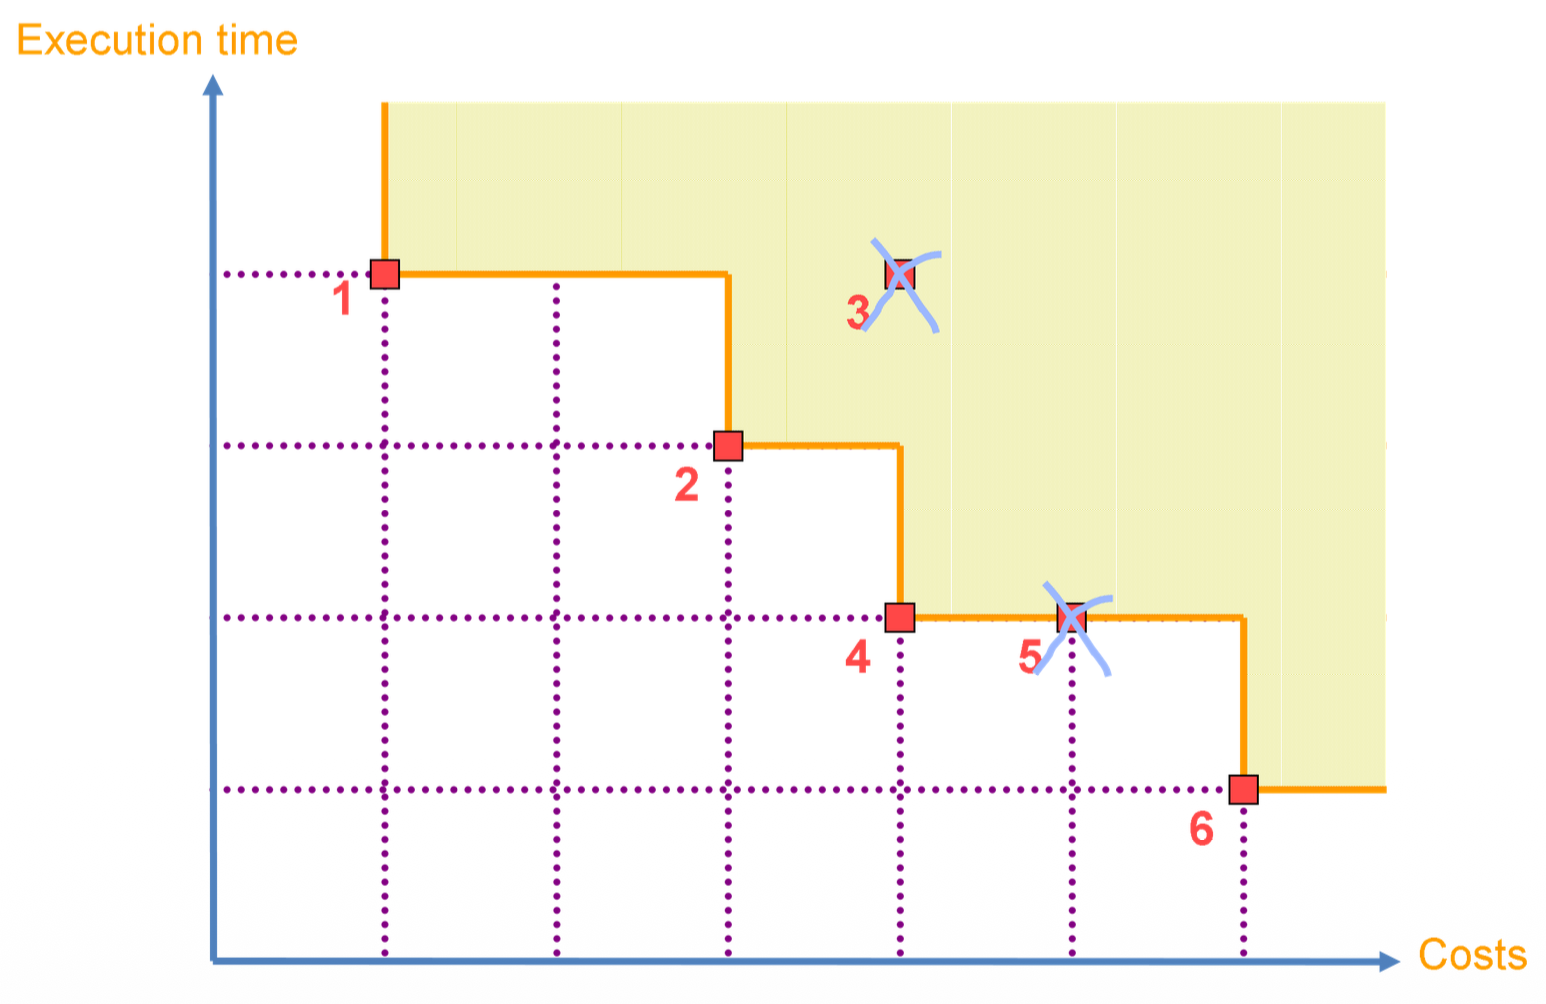
\includegraphics[width=0.5\textwidth]{images/Design_space_exploration.png}
		\caption{Pareto optimal design space exploration}
	\end{center}
\end{figure}











